\documentclass[11pt,a4paper]{article}
\usepackage{TeX_definitions}
\geometry{left=2.4cm,right=2.4cm,top=2.4cm,bottom=2.4cm}
\graphicspath{{figures/}}
\hypersetup{colorlinks=true,linkcolor=blue,citecolor=blue,urlcolor=blue}

\title{Analysis 4-4: is the local log-evidence heuristic genuinely a new family?}
\author{}
\date{\today}
\begin{document}
\maketitle

\section{Question}
Analysis 4-4 asks whether the proposed local log-evidence heuristic defines a new agent family or merely restates the shell-0 local model already present in the project.

\section{Method}
Standard graphical-model background and notation are treated in the usual way; see \cite{Koller2009}.


We formalised the heuristic as a sum of direct-neighbour log messages followed by exponentiation and normalisation. We then compared its outputs to $M_0$ over the full rooted library, and also simulated two deliberately non-equivalent distortions: neighbour-specific weighting and score clipping.

\section{Results}
The numerical result is unambiguous. The maximum absolute difference between the pure heuristic and $M_0$ was 0.0, and the mean JS divergence to $M_0$ was 0.0. By construction, the weighted and clipped variants departed from $M_0$ (mean JS 0.0114248243 and 0.014439751, respectively).

\begin{figure}[H]
\centering
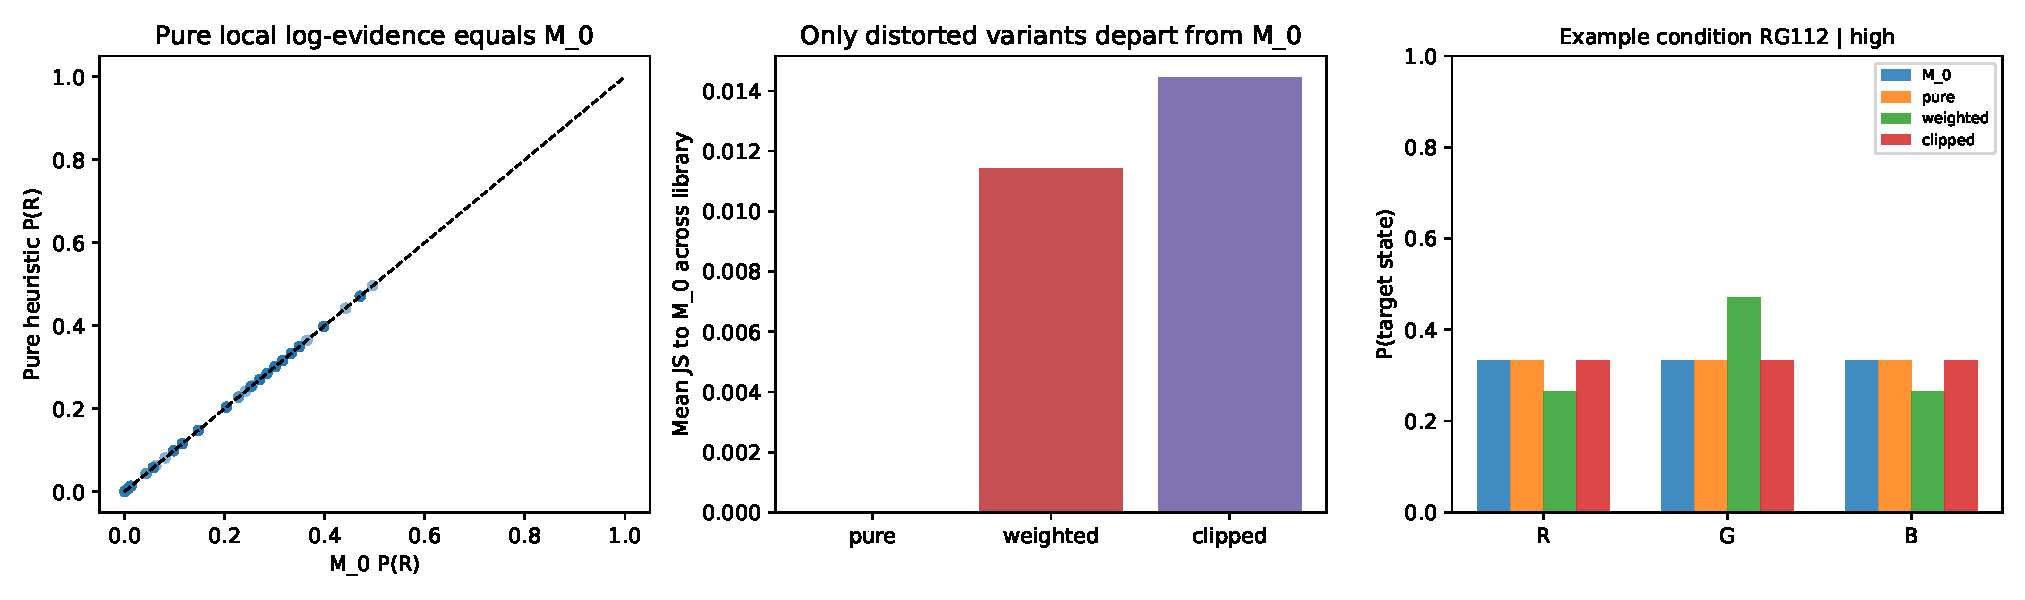
\includegraphics[width=\textwidth]{analysis-4-4_fig1_equivalence_check.pdf}
\caption{The pure local log-evidence heuristic lies exactly on top of $M_0$, whereas distorted variants deviate.}
\end{figure}

\section{Conclusions against the TODO}
\begin{enumerate}
    \item The heuristic now has a precise mathematical statement.
    \item Under the standard normalised readout, it is exactly $M_0$.
    \item Only weighted, clipped, or response-distorted variants are genuinely distinct.
    \item The pure heuristic should therefore be removed from the core family set rather than treated as a seventh inference family.
\end{enumerate}

\bibliographystyle{apalike}
\bibliography{../../manuscript/library}
\end{document}
